\chapter{PENDAHULUAN}

\section{Latar Belakang}
Bagian ini secara umum berisi latar belakang dan alasan penulis memilih objek penelitian. Uraian dimulai dengan penjelasan mengenai hal yang bersifat umum terkait dengan topik Tugas Akhir (TA), kemudian diarahkan kepada hal yang lebih khusus yaitu judul proposal TA. Objek yang akan diteliti harus dijelaskan secara konkret sebagai pengantar menuju permasalahan, dan sebagai hasil kajian/studi terdahulu/hasil analisis atas data sekunder, tentang obyek yang akan diteliti/dirancang, disertai alasan mengapa masalah tersebut perlu diteliti baik secara teoritis maupun praktis. 
%pergantian paragraf
Latar belakang tugas akhir biasanya berisi gap analysis yang fungsinya untuk mengidentifikasi dan menjelaskan kesenjangan antara kondisi atau pengetahuan yang ada dengan kondisi ideal atau yang diinginkan. Dalam konteks penelitian, gap analysis membantu mengungkapkan area di mana penelitian sebelumnya belum memadai, atau ada aspek yang belum terjelaskan dengan baik. Dengan demikian, latar belakang tugas akhir menjelaskan mengapa penelitian ini penting dilakukan untuk mengisi kesenjangan tersebut, sekaligus membuktikan relevansi dan kontribusi dari penelitian yang diusulkan. Hal ini memperkuat argumen tentang nilai dan urgensi penelitian yang akan dilakukan. Tambahkan gambar apabila diperlukan. Contoh tampilan gambar dapat dilihat pada Gambar \ref{fig:kapasitor}.


\begin{figure}[h!]
    \centering
    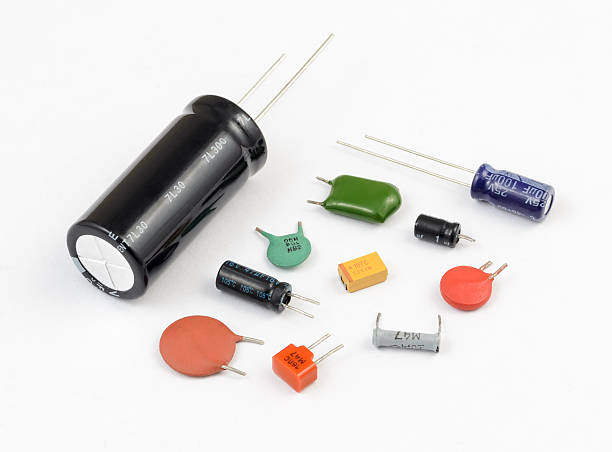
\includegraphics[width=0.7\textwidth]{gambar/kapasitor.jpg}
    \caption{Jenis Kapasitor di Dunia Elektro}
    \label{fig:kapasitor}
\end{figure}

\section{Rumusan Masalah}
Permasalahan penelitian harus dituliskan dalam bentuk deklaratif atau kalimat-kalimat pertanyaan yang tegas dan jelas. Masalah penelitian merupakan perumusan kesenjangan antara keadaan yang ada dengan keadaan yang ingin dicapai. Perumusan masalah dilakukan berdasarkan identifikasi masalah dan ruang lingkup penelitian yang akan dipecahkan. Perumusan masalah ini dituangkan dalam bentuk pertanyaan yang nantinya akan dijawab di dalam analisis masalah dengan menggunakan teori atau konsep yang relevan dan didukung oleh data pada pelaksanaan penelitian yang akan dilakukan. Dalam merumuskan masalah perlu dihindari mengemukakan banyak pertanyaan, yang artinya bahwa rumusan masalah tidak dituliskan dalam bentuk pertanyaan yang terlalu banyak jumlahnya.

\section{Batasan Masalah}
Ruang lingkup/pembatasan masalah dalam upaya memfokuskan penelitian yang akan dilakukan menjadi lebih terarah. Pembatasan dapat dilakukan dari segi keluasan, kedalaman, kemampuan peneliti dalam aspek tertentu, atau semua segi tersebut. Pembatasan harus disertai alasan atau argumentasi mengapa pembatasan masalah perlu dilakukan. Batasan masalah terkait dengan variable penelitian/variabel perancangan, variabel dan/atau parameter terhadap variabel penelitian/perancangan, dan/atau variabel/parameter yang diasumsikan sebagai parameter konstanta atau parameter yang diabaikan.

\section{Tujuan}
Tujuan penelitian/perancangan berisi uraian tentang tujuan penulis melakukan penelitian/perancangan, yaitu untuk menjawab pertanyaan yang telah dituliskan di dalam bagian perumusan masalah atau hasil yang akan dicapai atau jawaban permasalahan penelitian/perancangan. Tujuan penelitian/perancangan dapat dituliskan dalam serangkaian tujuan, yang merupakan tujuan yang lebih spesifik, yang mendukung tujuan penelitian/perancangan. Pada bagian tujuan ini biasanya dapat dituliskan dalam bentuk poin-poin seperti contoh berikut:
\begin{enumerate}[leftmargin=1.25cm] % sejajar dengan paragraf/sub-bab
    \item Untuk mengembangkan...;
    \item Untuk mengidentifikasi...;
    \item Untuk mengukur...;
    \item Untuk menentukan...;
    \item Untuk membandingkan.... 
\end{enumerate}
\section{Manfaat}
Pada bagian ini diuraikan secara singkat tetapi jelas kontribusi hasil penelitian/perancangan terhadap pengembangan bidang ilmu, teknologi, seni dan atau terhadap pemecahan persoalan pembangunan, dan atau terhadap pengembangan institusi.
